% Options for packages loaded elsewhere
\PassOptionsToPackage{unicode}{hyperref}
\PassOptionsToPackage{hyphens}{url}
\PassOptionsToPackage{dvipsnames,svgnames,x11names}{xcolor}
%
\documentclass[
]{agujournal2019}

\usepackage{amsmath,amssymb}
\usepackage{iftex}
\ifPDFTeX
  \usepackage[T1]{fontenc}
  \usepackage[utf8]{inputenc}
  \usepackage{textcomp} % provide euro and other symbols
\else % if luatex or xetex
  \usepackage{unicode-math}
  \defaultfontfeatures{Scale=MatchLowercase}
  \defaultfontfeatures[\rmfamily]{Ligatures=TeX,Scale=1}
\fi
\usepackage{lmodern}
\ifPDFTeX\else  
    % xetex/luatex font selection
\fi
% Use upquote if available, for straight quotes in verbatim environments
\IfFileExists{upquote.sty}{\usepackage{upquote}}{}
\IfFileExists{microtype.sty}{% use microtype if available
  \usepackage[]{microtype}
  \UseMicrotypeSet[protrusion]{basicmath} % disable protrusion for tt fonts
}{}
\makeatletter
\@ifundefined{KOMAClassName}{% if non-KOMA class
  \IfFileExists{parskip.sty}{%
    \usepackage{parskip}
  }{% else
    \setlength{\parindent}{0pt}
    \setlength{\parskip}{6pt plus 2pt minus 1pt}}
}{% if KOMA class
  \KOMAoptions{parskip=half}}
\makeatother
\usepackage{xcolor}
\setlength{\emergencystretch}{3em} % prevent overfull lines
\setcounter{secnumdepth}{5}
% Make \paragraph and \subparagraph free-standing
\makeatletter
\ifx\paragraph\undefined\else
  \let\oldparagraph\paragraph
  \renewcommand{\paragraph}{
    \@ifstar
      \xxxParagraphStar
      \xxxParagraphNoStar
  }
  \newcommand{\xxxParagraphStar}[1]{\oldparagraph*{#1}\mbox{}}
  \newcommand{\xxxParagraphNoStar}[1]{\oldparagraph{#1}\mbox{}}
\fi
\ifx\subparagraph\undefined\else
  \let\oldsubparagraph\subparagraph
  \renewcommand{\subparagraph}{
    \@ifstar
      \xxxSubParagraphStar
      \xxxSubParagraphNoStar
  }
  \newcommand{\xxxSubParagraphStar}[1]{\oldsubparagraph*{#1}\mbox{}}
  \newcommand{\xxxSubParagraphNoStar}[1]{\oldsubparagraph{#1}\mbox{}}
\fi
\makeatother

\usepackage{color}
\usepackage{fancyvrb}
\newcommand{\VerbBar}{|}
\newcommand{\VERB}{\Verb[commandchars=\\\{\}]}
\DefineVerbatimEnvironment{Highlighting}{Verbatim}{commandchars=\\\{\}}
% Add ',fontsize=\small' for more characters per line
\usepackage{framed}
\definecolor{shadecolor}{RGB}{241,243,245}
\newenvironment{Shaded}{\begin{snugshade}}{\end{snugshade}}
\newcommand{\AlertTok}[1]{\textcolor[rgb]{0.68,0.00,0.00}{#1}}
\newcommand{\AnnotationTok}[1]{\textcolor[rgb]{0.37,0.37,0.37}{#1}}
\newcommand{\AttributeTok}[1]{\textcolor[rgb]{0.40,0.45,0.13}{#1}}
\newcommand{\BaseNTok}[1]{\textcolor[rgb]{0.68,0.00,0.00}{#1}}
\newcommand{\BuiltInTok}[1]{\textcolor[rgb]{0.00,0.23,0.31}{#1}}
\newcommand{\CharTok}[1]{\textcolor[rgb]{0.13,0.47,0.30}{#1}}
\newcommand{\CommentTok}[1]{\textcolor[rgb]{0.37,0.37,0.37}{#1}}
\newcommand{\CommentVarTok}[1]{\textcolor[rgb]{0.37,0.37,0.37}{\textit{#1}}}
\newcommand{\ConstantTok}[1]{\textcolor[rgb]{0.56,0.35,0.01}{#1}}
\newcommand{\ControlFlowTok}[1]{\textcolor[rgb]{0.00,0.23,0.31}{\textbf{#1}}}
\newcommand{\DataTypeTok}[1]{\textcolor[rgb]{0.68,0.00,0.00}{#1}}
\newcommand{\DecValTok}[1]{\textcolor[rgb]{0.68,0.00,0.00}{#1}}
\newcommand{\DocumentationTok}[1]{\textcolor[rgb]{0.37,0.37,0.37}{\textit{#1}}}
\newcommand{\ErrorTok}[1]{\textcolor[rgb]{0.68,0.00,0.00}{#1}}
\newcommand{\ExtensionTok}[1]{\textcolor[rgb]{0.00,0.23,0.31}{#1}}
\newcommand{\FloatTok}[1]{\textcolor[rgb]{0.68,0.00,0.00}{#1}}
\newcommand{\FunctionTok}[1]{\textcolor[rgb]{0.28,0.35,0.67}{#1}}
\newcommand{\ImportTok}[1]{\textcolor[rgb]{0.00,0.46,0.62}{#1}}
\newcommand{\InformationTok}[1]{\textcolor[rgb]{0.37,0.37,0.37}{#1}}
\newcommand{\KeywordTok}[1]{\textcolor[rgb]{0.00,0.23,0.31}{\textbf{#1}}}
\newcommand{\NormalTok}[1]{\textcolor[rgb]{0.00,0.23,0.31}{#1}}
\newcommand{\OperatorTok}[1]{\textcolor[rgb]{0.37,0.37,0.37}{#1}}
\newcommand{\OtherTok}[1]{\textcolor[rgb]{0.00,0.23,0.31}{#1}}
\newcommand{\PreprocessorTok}[1]{\textcolor[rgb]{0.68,0.00,0.00}{#1}}
\newcommand{\RegionMarkerTok}[1]{\textcolor[rgb]{0.00,0.23,0.31}{#1}}
\newcommand{\SpecialCharTok}[1]{\textcolor[rgb]{0.37,0.37,0.37}{#1}}
\newcommand{\SpecialStringTok}[1]{\textcolor[rgb]{0.13,0.47,0.30}{#1}}
\newcommand{\StringTok}[1]{\textcolor[rgb]{0.13,0.47,0.30}{#1}}
\newcommand{\VariableTok}[1]{\textcolor[rgb]{0.07,0.07,0.07}{#1}}
\newcommand{\VerbatimStringTok}[1]{\textcolor[rgb]{0.13,0.47,0.30}{#1}}
\newcommand{\WarningTok}[1]{\textcolor[rgb]{0.37,0.37,0.37}{\textit{#1}}}

\providecommand{\tightlist}{%
  \setlength{\itemsep}{0pt}\setlength{\parskip}{0pt}}\usepackage{longtable,booktabs,array}
\usepackage{calc} % for calculating minipage widths
% Correct order of tables after \paragraph or \subparagraph
\usepackage{etoolbox}
\makeatletter
\patchcmd\longtable{\par}{\if@noskipsec\mbox{}\fi\par}{}{}
\makeatother
% Allow footnotes in longtable head/foot
\IfFileExists{footnotehyper.sty}{\usepackage{footnotehyper}}{\usepackage{footnote}}
\makesavenoteenv{longtable}
\usepackage{graphicx}
\makeatletter
\newsavebox\pandoc@box
\newcommand*\pandocbounded[1]{% scales image to fit in text height/width
  \sbox\pandoc@box{#1}%
  \Gscale@div\@tempa{\textheight}{\dimexpr\ht\pandoc@box+\dp\pandoc@box\relax}%
  \Gscale@div\@tempb{\linewidth}{\wd\pandoc@box}%
  \ifdim\@tempb\p@<\@tempa\p@\let\@tempa\@tempb\fi% select the smaller of both
  \ifdim\@tempa\p@<\p@\scalebox{\@tempa}{\usebox\pandoc@box}%
  \else\usebox{\pandoc@box}%
  \fi%
}
% Set default figure placement to htbp
\def\fps@figure{htbp}
\makeatother
% definitions for citeproc citations
\NewDocumentCommand\citeproctext{}{}
\NewDocumentCommand\citeproc{mm}{%
  \begingroup\def\citeproctext{#2}\cite{#1}\endgroup}
\makeatletter
 % allow citations to break across lines
 \let\@cite@ofmt\@firstofone
 % avoid brackets around text for \cite:
 \def\@biblabel#1{}
 \def\@cite#1#2{{#1\if@tempswa , #2\fi}}
\makeatother
\newlength{\cslhangindent}
\setlength{\cslhangindent}{1.5em}
\newlength{\csllabelwidth}
\setlength{\csllabelwidth}{3em}
\newenvironment{CSLReferences}[2] % #1 hanging-indent, #2 entry-spacing
 {\begin{list}{}{%
  \setlength{\itemindent}{0pt}
  \setlength{\leftmargin}{0pt}
  \setlength{\parsep}{0pt}
  % turn on hanging indent if param 1 is 1
  \ifodd #1
   \setlength{\leftmargin}{\cslhangindent}
   \setlength{\itemindent}{-1\cslhangindent}
  \fi
  % set entry spacing
  \setlength{\itemsep}{#2\baselineskip}}}
 {\end{list}}
\usepackage{calc}
\newcommand{\CSLBlock}[1]{\hfill\break\parbox[t]{\linewidth}{\strut\ignorespaces#1\strut}}
\newcommand{\CSLLeftMargin}[1]{\parbox[t]{\csllabelwidth}{\strut#1\strut}}
\newcommand{\CSLRightInline}[1]{\parbox[t]{\linewidth - \csllabelwidth}{\strut#1\strut}}
\newcommand{\CSLIndent}[1]{\hspace{\cslhangindent}#1}

\usepackage{url} %this package should fix any errors with URLs in refs.
\usepackage{lineno}
\usepackage[inline]{trackchanges} %for better track changes. finalnew option will compile document with changes incorporated.
\usepackage{soul}
\linenumbers
\makeatletter
\@ifpackageloaded{caption}{}{\usepackage{caption}}
\AtBeginDocument{%
\ifdefined\contentsname
  \renewcommand*\contentsname{Table of contents}
\else
  \newcommand\contentsname{Table of contents}
\fi
\ifdefined\listfigurename
  \renewcommand*\listfigurename{List of Figures}
\else
  \newcommand\listfigurename{List of Figures}
\fi
\ifdefined\listtablename
  \renewcommand*\listtablename{List of Tables}
\else
  \newcommand\listtablename{List of Tables}
\fi
\ifdefined\figurename
  \renewcommand*\figurename{Figure}
\else
  \newcommand\figurename{Figure}
\fi
\ifdefined\tablename
  \renewcommand*\tablename{Table}
\else
  \newcommand\tablename{Table}
\fi
}
\@ifpackageloaded{float}{}{\usepackage{float}}
\floatstyle{ruled}
\@ifundefined{c@chapter}{\newfloat{codelisting}{h}{lop}}{\newfloat{codelisting}{h}{lop}[chapter]}
\floatname{codelisting}{Listing}
\newcommand*\listoflistings{\listof{codelisting}{List of Listings}}
\makeatother
\makeatletter
\makeatother
\makeatletter
\@ifpackageloaded{caption}{}{\usepackage{caption}}
\@ifpackageloaded{subcaption}{}{\usepackage{subcaption}}
\makeatother

\usepackage{bookmark}

\IfFileExists{xurl.sty}{\usepackage{xurl}}{} % add URL line breaks if available
\urlstyle{same} % disable monospaced font for URLs
\hypersetup{
  pdftitle={Supply Chain Data Analytics},
  colorlinks=true,
  linkcolor={blue},
  filecolor={Maroon},
  citecolor={Blue},
  urlcolor={Blue},
  pdfcreator={LaTeX via pandoc}}


\journalname{Earth and Space Science}

\draftfalse

\begin{document}
\title{Supply Chain Data Analytics}

\authors{Stan Brouwer\affil{1}, Liz Chan\affil{2}, Maaike
Lamberst\affil{3}, Niek Schroor\affil{4}}
\affiliation{1}{Vrije Universiteit, }\affiliation{2}{Master
TSCM, }\affiliation{3}{Supply Chain Data
analysis, }\affiliation{4}{Group 10, }
\correspondingauthor{Stan Brouwer}{}







We analyze, forecast and interpret the
\href{https://public.tableau.com/app/sample-data/sample_-_superstore.xls}{Superstore
sales} provided by
\href{https://public.tableau.com/app/learn/sample-data}{Tableau} using
different statistical and machine learning methods.

We describe our work in the PDF version. However, we would like to
recommend reading our quarto manuscript \emph{here} as it contains the
\textbf{relevant} R code in the Article Notebook.

\subsection{Data Pre-processing}\label{data-pre-processing}

The superstore data set we selected is of high quality. Thus we do the
required data pre-processing, but included the hypothetical steps we
would take were our data of lower quality to communicate our
understanding of the data pre-processing process.

We took the following pre-processing steps:

\begin{itemize}
\tightlist
\item
  Improved column names by removing whitespaces
\item
  Removed the Row\_ID column as it can be inferred by it's index
\item
  Removed all columns with a single unique value, as storing these would
  be
  \href{https://few.vu.nl/~molenaar/courses/StatR/chapters/B-06-raw_data.html}{redundant}
\item
  Ensured machine-readable date formats in yyyy-mm-dd as these usually
  differ per locale.
\item
  Ensured proper decimal separators
\item
  calculated the number of missing values (both NA and empty string
  ``\,``) per column.
\end{itemize}

\begin{verbatim}
[1] "No missing values"
\end{verbatim}

\textsubscript{Source:
\href{https://SJbrou.github.io/Supply_Chain_Data_Analysis/index.qmd.html}{Article
Notebook}}

We also ran some descriptive statistics to check unlikely or impossible
values, outliers, means, etc.

\begin{verbatim}
# A tibble: 5 x 19
  Order_ID     Order_Date Ship_Date  Ship_Mode Customer_ID Customer_Name Segment
  <chr>        <date>     <date>     <chr>     <chr>       <chr>         <chr>  
1 CA-2016-152~ 2016-11-08 2016-11-11 Second C~ CG-12520    Claire Gute   Consum~
2 CA-2016-152~ 2016-11-08 2016-11-11 Second C~ CG-12520    Claire Gute   Consum~
3 CA-2016-138~ 2016-06-12 2016-06-16 Second C~ DV-13045    Darrin Van H~ Corpor~
4 US-2015-108~ 2015-10-11 2015-10-18 Standard~ SO-20335    Sean O'Donne~ Consum~
5 US-2015-108~ 2015-10-11 2015-10-18 Standard~ SO-20335    Sean O'Donne~ Consum~
# i 12 more variables: City <chr>, State <chr>, Postal_Code <dbl>,
#   Region <chr>, Product_ID <chr>, Category <chr>, `Sub-Category` <chr>,
#   Product_Name <chr>, Sales <dbl>, Quantity <dbl>, Discount <dbl>,
#   Profit <dbl>
\end{verbatim}

\textsubscript{Source:
\href{https://SJbrou.github.io/Supply_Chain_Data_Analysis/index.qmd.html}{Article
Notebook}}

There is some more processing to do, such as removing outliers. However,
by doing so we impose our own assumptions on the data (possibly the
outliers are actual sales?). We will visualize and qualitatively
evaluate the data first, and then decide what other processing steps to
take.

\begin{longtable}[]{@{}
  >{\raggedright\arraybackslash}p{(\linewidth - 36\tabcolsep) * \real{0.0540}}
  >{\raggedright\arraybackslash}p{(\linewidth - 36\tabcolsep) * \real{0.0396}}
  >{\raggedright\arraybackslash}p{(\linewidth - 36\tabcolsep) * \real{0.0396}}
  >{\raggedright\arraybackslash}p{(\linewidth - 36\tabcolsep) * \real{0.0540}}
  >{\raggedright\arraybackslash}p{(\linewidth - 36\tabcolsep) * \real{0.0432}}
  >{\raggedright\arraybackslash}p{(\linewidth - 36\tabcolsep) * \real{0.0576}}
  >{\raggedright\arraybackslash}p{(\linewidth - 36\tabcolsep) * \real{0.0360}}
  >{\raggedright\arraybackslash}p{(\linewidth - 36\tabcolsep) * \real{0.0576}}
  >{\raggedright\arraybackslash}p{(\linewidth - 36\tabcolsep) * \real{0.0396}}
  >{\raggedleft\arraybackslash}p{(\linewidth - 36\tabcolsep) * \real{0.0432}}
  >{\raggedright\arraybackslash}p{(\linewidth - 36\tabcolsep) * \real{0.0252}}
  >{\raggedright\arraybackslash}p{(\linewidth - 36\tabcolsep) * \real{0.0576}}
  >{\raggedright\arraybackslash}p{(\linewidth - 36\tabcolsep) * \real{0.0576}}
  >{\raggedright\arraybackslash}p{(\linewidth - 36\tabcolsep) * \real{0.0468}}
  >{\raggedright\arraybackslash}p{(\linewidth - 36\tabcolsep) * \real{0.2158}}
  >{\raggedleft\arraybackslash}p{(\linewidth - 36\tabcolsep) * \real{0.0324}}
  >{\raggedleft\arraybackslash}p{(\linewidth - 36\tabcolsep) * \real{0.0324}}
  >{\raggedleft\arraybackslash}p{(\linewidth - 36\tabcolsep) * \real{0.0324}}
  >{\raggedleft\arraybackslash}p{(\linewidth - 36\tabcolsep) * \real{0.0360}}@{}}
\caption{First 5 Rows of the Data}\tabularnewline
\toprule\noalign{}
\begin{minipage}[b]{\linewidth}\raggedright
Order\_ID
\end{minipage} & \begin{minipage}[b]{\linewidth}\raggedright
Order\_Date
\end{minipage} & \begin{minipage}[b]{\linewidth}\raggedright
Ship\_Date
\end{minipage} & \begin{minipage}[b]{\linewidth}\raggedright
Ship\_Mode
\end{minipage} & \begin{minipage}[b]{\linewidth}\raggedright
Customer\_ID
\end{minipage} & \begin{minipage}[b]{\linewidth}\raggedright
Customer\_Name
\end{minipage} & \begin{minipage}[b]{\linewidth}\raggedright
Segment
\end{minipage} & \begin{minipage}[b]{\linewidth}\raggedright
City
\end{minipage} & \begin{minipage}[b]{\linewidth}\raggedright
State
\end{minipage} & \begin{minipage}[b]{\linewidth}\raggedleft
Postal\_Code
\end{minipage} & \begin{minipage}[b]{\linewidth}\raggedright
Region
\end{minipage} & \begin{minipage}[b]{\linewidth}\raggedright
Product\_ID
\end{minipage} & \begin{minipage}[b]{\linewidth}\raggedright
Category
\end{minipage} & \begin{minipage}[b]{\linewidth}\raggedright
Sub-Category
\end{minipage} & \begin{minipage}[b]{\linewidth}\raggedright
Product\_Name
\end{minipage} & \begin{minipage}[b]{\linewidth}\raggedleft
Sales
\end{minipage} & \begin{minipage}[b]{\linewidth}\raggedleft
Quantity
\end{minipage} & \begin{minipage}[b]{\linewidth}\raggedleft
Discount
\end{minipage} & \begin{minipage}[b]{\linewidth}\raggedleft
Profit
\end{minipage} \\
\midrule\noalign{}
\endfirsthead
\toprule\noalign{}
\begin{minipage}[b]{\linewidth}\raggedright
Order\_ID
\end{minipage} & \begin{minipage}[b]{\linewidth}\raggedright
Order\_Date
\end{minipage} & \begin{minipage}[b]{\linewidth}\raggedright
Ship\_Date
\end{minipage} & \begin{minipage}[b]{\linewidth}\raggedright
Ship\_Mode
\end{minipage} & \begin{minipage}[b]{\linewidth}\raggedright
Customer\_ID
\end{minipage} & \begin{minipage}[b]{\linewidth}\raggedright
Customer\_Name
\end{minipage} & \begin{minipage}[b]{\linewidth}\raggedright
Segment
\end{minipage} & \begin{minipage}[b]{\linewidth}\raggedright
City
\end{minipage} & \begin{minipage}[b]{\linewidth}\raggedright
State
\end{minipage} & \begin{minipage}[b]{\linewidth}\raggedleft
Postal\_Code
\end{minipage} & \begin{minipage}[b]{\linewidth}\raggedright
Region
\end{minipage} & \begin{minipage}[b]{\linewidth}\raggedright
Product\_ID
\end{minipage} & \begin{minipage}[b]{\linewidth}\raggedright
Category
\end{minipage} & \begin{minipage}[b]{\linewidth}\raggedright
Sub-Category
\end{minipage} & \begin{minipage}[b]{\linewidth}\raggedright
Product\_Name
\end{minipage} & \begin{minipage}[b]{\linewidth}\raggedleft
Sales
\end{minipage} & \begin{minipage}[b]{\linewidth}\raggedleft
Quantity
\end{minipage} & \begin{minipage}[b]{\linewidth}\raggedleft
Discount
\end{minipage} & \begin{minipage}[b]{\linewidth}\raggedleft
Profit
\end{minipage} \\
\midrule\noalign{}
\endhead
\bottomrule\noalign{}
\endlastfoot
CA-2016-152156 & 2016-11-08 & 2016-11-11 & Second Class & CG-12520 &
Claire Gute & Consumer & Henderson & Kentucky & 42420 & South &
FUR-BO-10001798 & Furniture & Bookcases & Bush Somerset Collection
Bookcase & 261.9600 & 2 & 0.00 & 41.9136 \\
CA-2016-152156 & 2016-11-08 & 2016-11-11 & Second Class & CG-12520 &
Claire Gute & Consumer & Henderson & Kentucky & 42420 & South &
FUR-CH-10000454 & Furniture & Chairs & Hon Deluxe Fabric Upholstered
Stacking Chairs, Rounded Back & 731.9400 & 3 & 0.00 & 219.5820 \\
CA-2016-138688 & 2016-06-12 & 2016-06-16 & Second Class & DV-13045 &
Darrin Van Huff & Corporate & Los Angeles & California & 90036 & West &
OFF-LA-10000240 & Office Supplies & Labels & Self-Adhesive Address
Labels for Typewriters by Universal & 14.6200 & 2 & 0.00 & 6.8714 \\
US-2015-108966 & 2015-10-11 & 2015-10-18 & Standard Class & SO-20335 &
Sean O'Donnell & Consumer & Fort Lauderdale & Florida & 33311 & South &
FUR-TA-10000577 & Furniture & Tables & Bretford CR4500 Series Slim
Rectangular Table & 957.5775 & 5 & 0.45 & -383.0310 \\
US-2015-108966 & 2015-10-11 & 2015-10-18 & Standard Class & SO-20335 &
Sean O'Donnell & Consumer & Fort Lauderdale & Florida & 33311 & South &
OFF-ST-10000760 & Office Supplies & Storage & Eldon Fold 'N Roll Cart
System & 22.3680 & 2 & 0.20 & 2.5164 \\
\end{longtable}

\textsubscript{Source:
\href{https://SJbrou.github.io/Supply_Chain_Data_Analysis/index.qmd.html}{Article
Notebook}}

\subsection{Section}\label{section}

This is a simple placeholder for the manuscript's main document
(\textbf{knuth84?}).

\begin{Shaded}
\begin{Highlighting}[]
\DecValTok{1} \SpecialCharTok{+} \DecValTok{1}
\end{Highlighting}
\end{Shaded}

\begin{verbatim}
[1] 2
\end{verbatim}

\textsubscript{Source:
\href{https://SJbrou.github.io/Supply_Chain_Data_Analysis/index.qmd.html}{Article
Notebook}}

\subsection{Introduction}\label{introduction}

\textsubscript{Source:
\href{https://SJbrou.github.io/Supply_Chain_Data_Analysis/index.qmd.html}{Article
Notebook}}

\phantomsection\label{cell-fig-timeline}
\begin{figure}[H]

\centering{

\pandocbounded{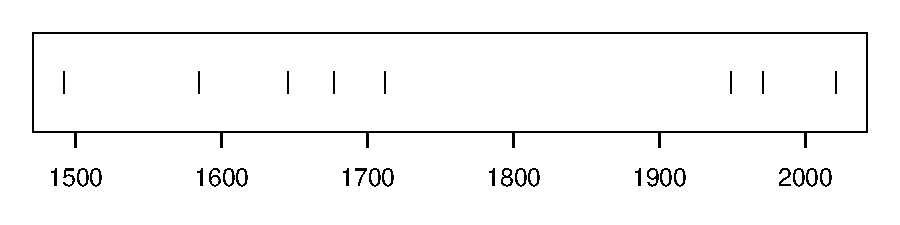
\includegraphics[keepaspectratio]{index_files/figure-pdf/fig-timeline-1.pdf}}

}

\caption{\label{fig-timeline}Timeline of recent earthquakes on La Palma}

\end{figure}%

\textsubscript{Source:
\href{https://SJbrou.github.io/Supply_Chain_Data_Analysis/index.qmd.html}{Article
Notebook}}

\textsubscript{Source:
\href{https://SJbrou.github.io/Supply_Chain_Data_Analysis/index.qmd.html}{Article
Notebook}}

Based on data up to and including 1971, eruptions on La Palma happen
every 79.8 years on average.

Studies of the magma systems feeding the volcano, such as Marrero et al.
(2019), have proposed that there are two main magma reservoirs feeding
the Cumbre Vieja volcano; one in the mantle (30-40km depth) which
charges and in turn feeds a shallower crustal reservoir (10-20km depth).

Eight eruptions have been recorded since the late 1400s
(Figure~\ref{fig-timeline}).

Data and methods are discussed in Section~\ref{sec-data-methods}.

Let \(x\) denote the number of eruptions in a year. Then, \(x\) can be
modeled by a Poisson distribution

\begin{equation}\phantomsection\label{eq-poisson}{
p(x) = \frac{e^{-\lambda} \lambda^{x}}{x !}
}\end{equation}

where \(\lambda\) is the rate of eruptions per year. Using
Equation~\ref{eq-poisson}, the probability of an eruption in the next
\(t\) years can be calculated.

\begin{longtable}[]{@{}ll@{}}
\caption{Recent historic eruptions on La
Palma}\label{tbl-history}\tabularnewline
\toprule\noalign{}
Name & Year \\
\midrule\noalign{}
\endfirsthead
\toprule\noalign{}
Name & Year \\
\midrule\noalign{}
\endhead
\bottomrule\noalign{}
\endlastfoot
Current & 2021 \\
Teneguía & 1971 \\
Nambroque & 1949 \\
El Charco & 1712 \\
Volcán San Antonio & 1677 \\
Volcán San Martin & 1646 \\
Tajuya near El Paso & 1585 \\
Montaña Quemada & 1492 \\
\end{longtable}

Table~\ref{tbl-history} summarises the eruptions recorded since the
colonization of the islands by Europeans in the late 1400s.

\begin{figure}

\centering{

\pandocbounded{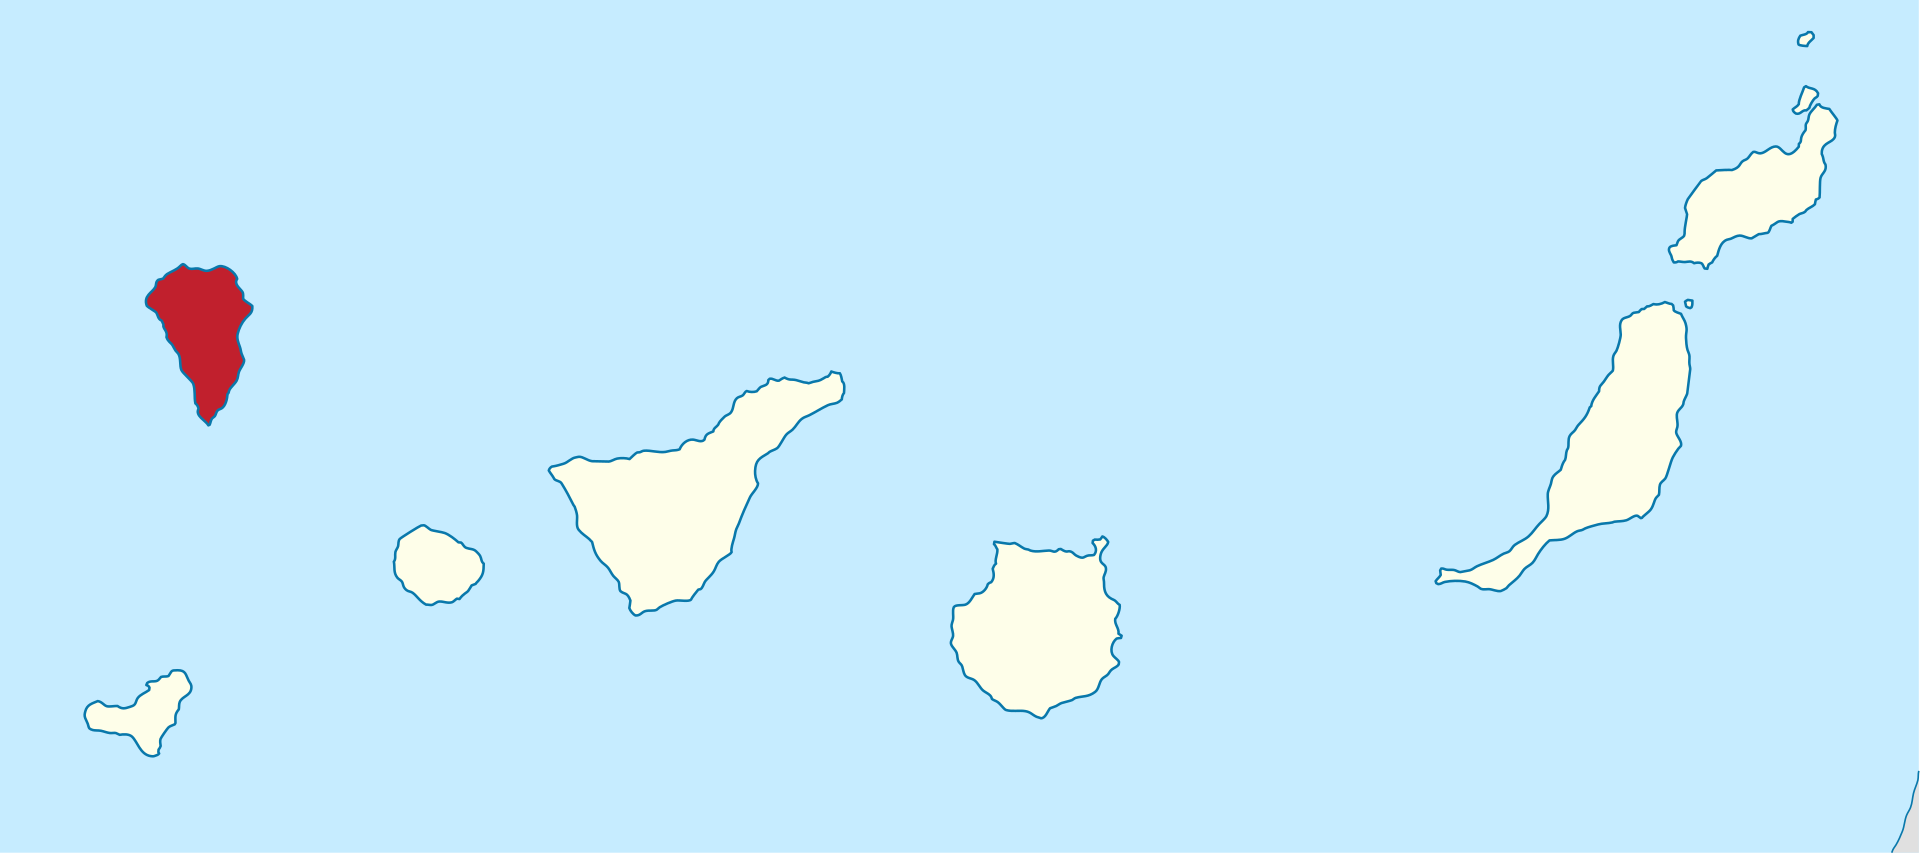
\includegraphics[keepaspectratio]{images/la-palma-map.png}}

}

\caption{\label{fig-map}Map of La Palma}

\end{figure}%

La Palma is one of the west most islands in the Volcanic Archipelago of
the Canary Islands (Figure~\ref{fig-map}).

\begin{figure}[H]

\centering{

\pandocbounded{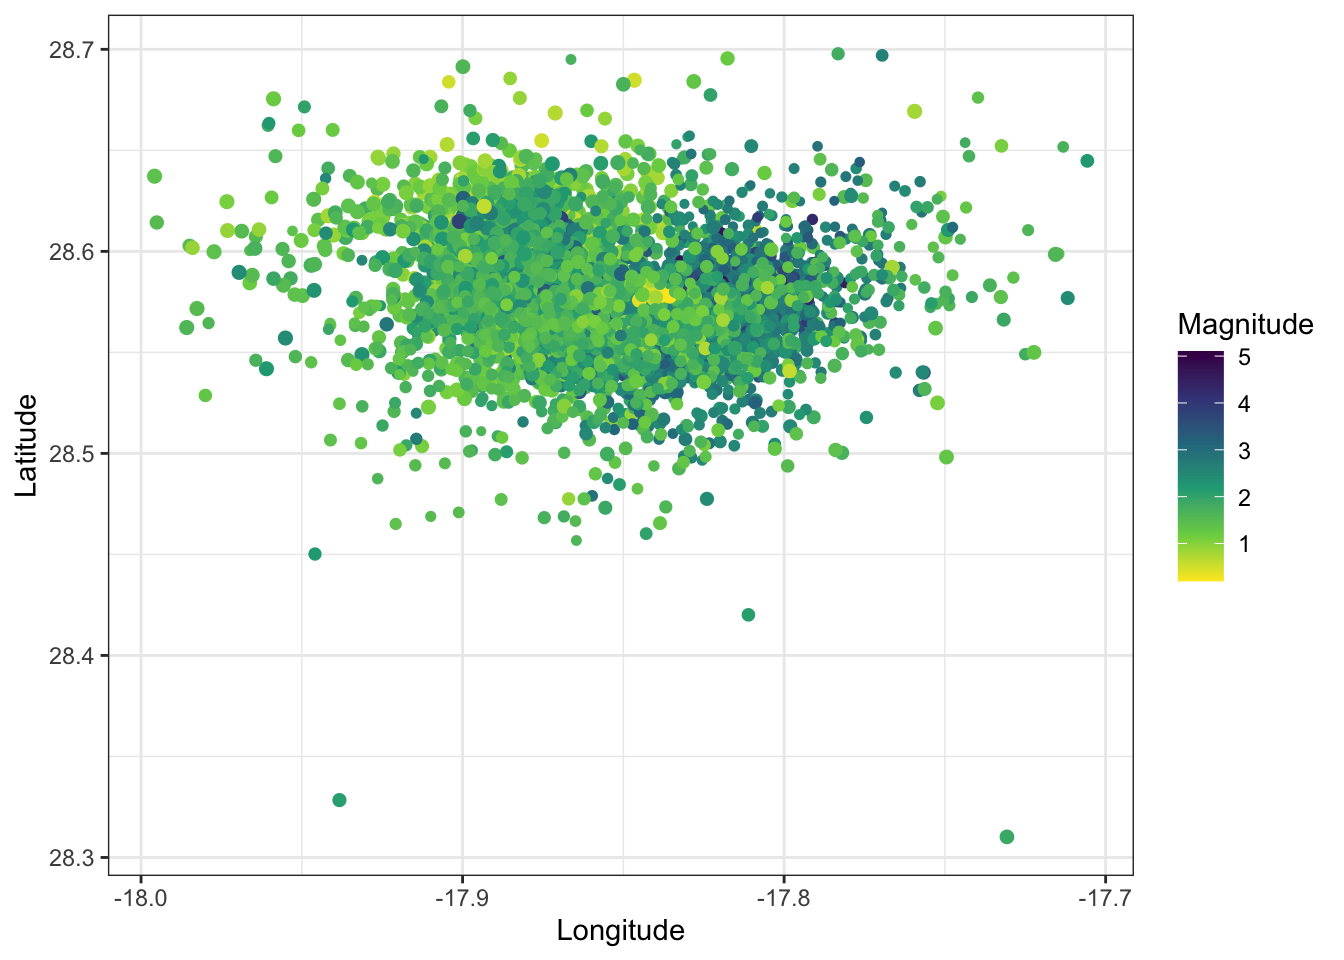
\includegraphics[keepaspectratio]{index_files/figure-latex/notebooks-explore-earthquakes-fig-spatial-plot-output-1.png}}

}

\caption{\label{fig-spatial-plot}Locations of earthquakes on La Palma
since 2017}

\end{figure}%

\textsubscript{Source:
\href{https://SJbrou.github.io/Supply_Chain_Data_Analysis/notebooks/explore-earthquakes-preview.html\#cell-fig-spatial-plot}{Explore
Earthquakes}}

Figure~\ref{fig-spatial-plot} shows the location of recent Earthquakes
on La Palma.

\subsection{Data \& Methods}\label{sec-data-methods}

\subsection{Conclusion}\label{conclusion}

\subsection*{References}\label{references}
\addcontentsline{toc}{subsection}{References}

\phantomsection\label{refs}
\begin{CSLReferences}{1}{0}
\vspace{1em}

\bibitem[\citeproctext]{ref-marrero2019}
Marrero, J., García, A., Berrocoso, M., Llinares, Á., Rodríguez-Losada,
A., \& Ortiz, R. (2019). Strategies for the development of volcanic
hazard maps in monogenetic volcanic fields: The example of {La} {Palma}
({Canary} {Islands}). \emph{Journal of Applied Volcanology}, \emph{8}.
\url{https://doi.org/10.1186/s13617-019-0085-5}

\end{CSLReferences}




\end{document}
